
% !TEX root = ../foundations.tex







\section{Interaction with cubical structures}
\label{S: transversality}

In this section we bring in some auxiliary structures that will help us further develop geometric cohomology and its connections to singular cohomology. In particular, we equip our manifolds with smooth cubulations. Many of our results would apply just as well with the more familiar smooth triangulations, but we find cubulations to be more convenient. In particular, in \cite{FMS-flows} we have considered geometric cochains in the presence of cubulations, demonstrating how to obtain a fully-defined cochain-level cup product via intersection using certain flows developed in terms of the cubulation. Cup products in geometric cohomology will be discussed in the following section.

Smooth cubulations are analogous to smooth triangulations in that they involve a homeomorphism $M \cong |X|$ between a manifold $M$ and the geometric realization $|X|$ of a cubical complex $X$ such that the restriction to each cubical face is a smooth embedding. What is slightly different, aside from substituting cubes (i.e.\ copies of $\interval^k$) for simplices, is that cubical complexes are required to have a bit more structure than simplicial complexes, which can always be constructed just by gluing together simplices along faces. The issue is that any simplicial complex can be given a total ordering of its vertices, and this ordering provides a canonical identification between any simplicial face and the standard model simplex of the same dimension. By contrast, the natural combinatorial structure on the vertices of the standard cube is not a total ordering but rather a partial ordering. In particular, if we take the standard cube to be $\interval^k = [0,1]^k \subset \R^k$, then we have $v\leq w$ for two vertices if each coordinate of $v$ is less than or equal to the corresponding coordinate of $w$. There turn out to be spaces obtained from naively gluing cubes that do not support compatible partial orderings of this type. So rather when we speak of cubical complexes we will restrict ourselves to complexes that do admit such combinatorial data.
Consequently, each cubical $k$-face comes equipped with an identification with the standard $k$-cube, and hence also a standard orientation. As we will note below, smooth cubulations of this form exist for any smooth manifold. In the remainder of this work, ``cubulation'' will always mean a smooth cubulation.

Also analogously to simplicial complexes, cubical complexes possess algebraic cubical chain and cochain complexes and so cubical homology and cohomology that coincides with singular homology and cohomology\footnote{We will show below that cubical homology coincide with singular cubical homology, which coincide with simplicial singular homology by \cite{EM53}. As all of the involved chain complexes are free, the corresponding cohomologies are also isomorphic by basic homological algebra \cite[Theorem 45.5]{Mun84}.\label{FN: cubical and singular}}. Our primary goal in this section is to see that there are direct geometrically-defined isomorphisms between cubical (co)homology nd geometric (co)homology.

For this, we first provide some background on cubical complexes and cubical homology and cohomology in \cref{S: cubes,S: cubical cochains}. Then in \cref{S: cubical and geometric homology} we show that the obvious map that takes a face of a cube complex to its corresponding geometric chain induces an isomorphism from cubical homology to geometric homology. Next, in \cref{S: transverse cochains}, we consider those geometric cochains that are transverse to a given cubulation and show that their cohomology agrees with the geometric cohomology obtained without that constraint.

The motivation for our interest in cochains that are transverse to the cubulation is that they allow us to define an \textit{intersection map} $\mc I$ from these transverse geometric cochains to the cubical cochains. If $F$ is a face of the cubulation, $F^*$ its dual cochain, and $W$ is a geometric cochain of complementary dimension to $F$, then the coefficient of $F^*$ in $\mc I(W)$ is simply the geometric intersection number of $W$ with $F$. This intersection map is defined in \cref{S: intersection map}, which also contains our proof that the intersection map induces a cohomology isomorphism when $H^*(M)$ is finitely generated in each degree. To implement this proof, we include in \cref{S: dual cubes} a discussion of what we call ``central subdivisions'' of cubical complexes, which are analogous to barycentric subdivisions of simplicial complexes and allow us to construct the cubical dual cells to faces of the cubulation.


\subsection{Cubical complexes and cubulations}\label{S: cubes}




We begin by recalling some notation from \cite{FMS-flows}. In the context of cubical complexes we write the unit interval as $\interval = [0,1]$ and define the \textbf{standard $n$-cube} to be
\begin{equation*}
\interval^n = \big\{ (x_1, \dots, x_n) \in \R^n\ |\ 0 \leq x_i \leq 1 \big\}.
\end{equation*}
Denote $\{1, \dots, n\}$ by $\overline{n}$.

Given a partition $F = (F_0, F_{01}, F_1)$ of $\overline n$, it determines a \textbf{face} of $\interval^n$ given by
\begin{equation*}
\{(x_1, \dots, x_n) \in \interval^n\ |\ \forall \varepsilon \in \{0, 1\},\ i \in F_\varepsilon \Rightarrow x_i = \varepsilon\}.
\end{equation*}
We abuse notation and write $F$ for both the partition and its associated face. We refer to coordinates $x_i$ with $i \in F_{01}$ as \textbf{free} and to the others as \textbf{bound}.
The \textbf{dimension} of $F$ is its number of free coordinates, and as usual the faces of dimension $0$ and $1$ are called vertices and edges, respectively. The set of vertices of $\interval^n$ is denoted by $\vertices(\interval^n)$.

For $\varepsilon \in \{0, 1\}$ and $i \in \overline{n}$, we define maps $\delta_i^\varepsilon \colon \interval^{n-1} \to \interval^{n}$ by
\begin{align*}
\delta_i^\varepsilon(x_1, \dots, x_{n-1}) & = (x_1, \dots, x_{i-1}, \varepsilon, x_i, \dots, x_{n-1}).
\end{align*}
Any composition of these is referred to as a \textbf{face inclusion map}.

For $v \in \vertices(\interval^n)$ all coordinates are bound -- that is, $v_{01} = \emptyset$. Thus
 $v$ is determined by the partition of $\overline n$ into $v_0$ and $v_1$, so
we have a bijection from the set of vertices of $\interval^n$ to the power set $\mathcal P(\overline n)$ of $\overline n$, sending $v$ to $v_1$.
The inclusion relation in the power set induces a poset structure on $\vertices(\interval^n)$ given explicitly by
\begin{equation*}
v = (\epsilon_1, \dots, \epsilon_n) \leq w = (\eta_1, \dots, \eta_n) \iff \forall i,\ \epsilon_i \leq \eta_i.
\end{equation*}
We will freely use the identification of these two posets.
Face embedding maps induce order-preserving maps at the level of vertices.

An \textbf{interval subposet} of $\mathcal P(\overline n)$ is one of the form $[v, w] = \{u \in \mathcal P(\overline n)\ |\ v \leq u \leq w\}$ for a pair of vertices $v \leq w$. There is a canonical bijection between faces of $\interval^n$ and such subposets, associating to $[v, w]$ the face $F$ defined by $F_\varepsilon = \{i \in \overline{n}\ |\ v_i = w_i = \varepsilon\}$ for $\varepsilon \in \{0, 1\}$.

The posets $\{\mathcal P(\overline n)\}_{n \geq 1}$ play the role for cubical complexes that finite totally ordered sets play for simplicial complexes.
Recall for comparison that one definition of an abstract ordered simplicial complex is as a pair $(V, X)$, where $V$ is a poset and $X$ is a collection of subsets of $V$, each with an induced total order, such that all singletons are in $X$ and subsets of sets in $X$ are also in $X$.
We have the following cubical analogue.

\begin{definition}\label{D:cubical}
	A \textbf{cubical complex} $X$ is a collection $\{ \sigma \}$ of finite non-empty subsets of a poset
	$\vertices(X)$, together with, for each $\sigma \in X$, an order-preserving bijection $\iota_\sigma \colon \sigma \to \mathcal P(\overline n)$ for some $n$, such that:
	\begin{enumerate}
		\item For all $v \in \vertices(X)$, $\{v\} \in X$,
		\item For all $\sigma \in X$ and all $[u,w] \subset \mathcal P(\overline n)$ the set $\rho = \iota_\sigma^{-1}([u,w]) \in X$ and the following commutes
		\begin{equation*}
		\begin{tikzcd} [row sep = tiny, column sep = small]
		\sigma \arrow[rr, "\iota_\sigma"] && \mathcal P(\overline n) \\
		& [-5pt] {[}u,w{]} \arrow[ur, hook] & \\
		\rho \arrow[uu, hook] \arrow[rr, "\iota_\rho"'] && \mathcal P(\overline m). \arrow[ul, "\cong"'] \arrow[uu, dashed]
		\end{tikzcd}
		\end{equation*}
	\end{enumerate}
	We refer to an element $\sigma \in X$ as a \textbf{cube} or \textbf{face} of $X$, refer to $\iota_\sigma \colon \sigma \to \mathcal P(\overline{n})$ as its \textbf{characteristic map},
	and refer to $n$ as its \textbf{dimension}. If $\rho \subseteq \sigma \in X$, we say that $\rho$ is a \textbf{face} of $\sigma$ in $X$.
	We identify elements in $\vertices(X)$ with the singleton subsets in $X$, referring to them as vertices.
\end{definition}





In analogy with the usual terminology in the simplicial setting, one could call these ``ordered cubical complexes," but we only work with these and have seen little use elsewhere for the unordered version.
Our definition sits between cubical sets \cite{jardine2002cubical} and cellular subsets of the cubical lattice of $\R^\infty$ \cite{kaczynski2006computational}, analogously to the way that abstract ordered simplicial complexes sit between simplicial sets and simplicial complexes.
The following geometric realization construction makes our definition and the cubical lattice definition essentially equivalent. Just as is the case for simplicial complexes, faces in cubical complexes are completely determined by their vertices.

Consider the category defined by the inclusion poset of a cubical complex $X$ and the subcategory ${\tt Cube}$ of the category ${\tt Top}$ of topological spaces whose objects are the $n$-cubes, identified with $\interval^n$, and whose morphisms are face inclusions.
The characteristic maps of $X$ define a functor from its poset category to $\mathtt{Cube}$, and we define its \textbf{geometric realization} as the colimit of this functor.
A \textbf{cubical structure} or \textbf{cubulation} on a space $S$ is a homeomorphism $h \colon |X| \to S$ from the geometric realization of a cubical complex.
We abuse notation and write $h \circ \iota_{|\sigma|}$ simply as $\iota_\sigma$ for any $\sigma \in X$ when a cubical structure $h \colon |X| \to S$ is understood.

A smooth cubulation is one for which characteristic maps are smooth maps of manifolds with corners.
Smooth cubulations exist for any smooth manifold, as in the following construction of \cite{ShSh92}.
Start with a smooth triangulation (see for example \cite[Theorem 10.6]{MUNK66} for the existence of such).
Consider the cell complex that is dual to its barycentric subdivision. Intersecting those dual cells with each simplex in the triangulation provides a subdivision of the simplex into cells that are linearly isomorphic to cubes.
Moreover, starting with an ordered triangulation -- obtained for example by taking a barycentric subdivision -- such a cubical decomposition embeds cellularly into the cubical lattice of $\R^\infty$, and thus it is the geometric realization of a cubical complex.


\begin{figure}[h]
	\begin{subfigure}{.4\textwidth}
		\centering
		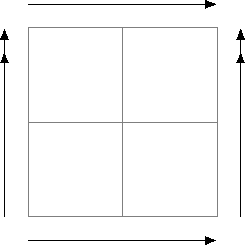
\includegraphics{figures/torus1.pdf}
		\caption{\textbf{Not} a cubulation of the torus}
	\end{subfigure}\qquad
	\begin{subfigure}{.4\textwidth}
		\centering
		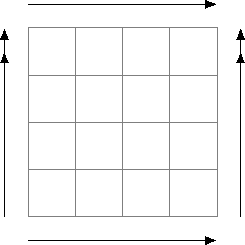
\includegraphics{figures/torus2.pdf}
		\caption{A cubulation of the torus}
	\end{subfigure}
	\caption{The first cellular decomposition of a torus pictured above does not represent the geometric realization of a cubical complex, as each square has the same set of vertices. On the right, each square can be coherently identified with the standard square with initial vertex in the lower left corner and final vertex in the upper right corner. Therefore, (B) depicts a cubical structure on the torus.}
	\label{F: cubical structure}
\end{figure}


\subsection{Cubical chains and cochains}\label{S: cubical cochains}

We can also define an ``algebraic realization" for a cubical complex in analogy to its geometric realization.
Let $K_*(\interval^1)$ be the usual cellular chain complex of the interval with integral coefficients.
Explicitly, $K_0(\interval^1)$ is generated by the vertices $[\underline{0}]$ and $[\underline{1}]$, and $K_1(\interval^1)$ is generated by the unique 1-dimensional face, denoted $[\underline{0},\underline{1}]$ in the interval subposet notation. The boundary map is $\bd [\underline{0},\underline{1}] = [\underline{1}]-[\underline{0}]$.

Let $K_*(\interval^n) = K_*(\interval^1)^{ \otimes n}$, with differential defined by the graded Leibniz rule.
Given a face inclusion $\delta_i^{\varepsilon} \colon \interval^n \to \interval^{n+1}$ the natural chain map $K_*(\delta_i^{\varepsilon}) \colon K_*(\interval^1)^{ \otimes n} \to K_*(\interval^1)^{ \otimes n+1}$ is defined on basis elements by
\begin{equation*}
x_1 \otimes \cdots \otimes x_n \mapsto
x_1 \otimes \cdots \otimes [\underline{\varepsilon}] \otimes \cdots \otimes x_n.
\end{equation*}
Regarding a cubical complex $X$ as a functor to $\mathtt{Cube}$, we can compose it with the chain functor above to obtain a functor to chain complexes.
The complex of \textbf{cubical chains} of $X$, denoted $K_*(X)$, is defined to be the colimit of this composition.
As one would expect, in each degree it is a free abelian group generated by the cubes of that dimension, and its boundary homomorphism sends the
generator associated to a cube to a sum of generators associated to its codimension-one faces with appropriate signs. By abuse, we use the same notation and terminology for an element in $X$, its geometric realization in $|X|$,
and the corresponding basis element in $K_*(X)$. Most commonly we will write $F$ and refer simply to a ``face of $X$.''

We note that for each $\interval^n$ we have the ordered set $\{\e_1, \dots, \e_n\}$ where $\e_i = \frac{\bd\ }{\bd x_i}$.
For any face $F$ of $\interval^n$, the ordered subset $\beta_F = \{\e_i\ |\ i \in F_{01}\}$ defines the \textbf{canonical orientation} of $F$. In forming the cubical complex $X$, these orientations are preserved, and so each face of $X$ carries an orientation. These orientations are compatible with our standard generators of $K_*(X)$ in the sense that if we identify $[0,1]^{ \otimes k}$ with $\interval^k$ with its standard orientation then, in the boundary formula, $k-1$ faces appear sign $1$ or $-1$ according to whether or not their standard orientations agree with the boundary orientation of $\interval^k$ as a manifold with corners.




The \textbf{cubical cochain complex} of $X$ (with $\Z$ coefficients) is the chain complex $K^*(X) = \Hom_\Z(K_*(X), \Z)$. If $F$ is a face of $X$, and correspondingly a generator of $K_*(X)$, then we will write $F^*$ for the dual, i.e.\ the generator of $K^*(X)$ such that $F^*(F) = 1$ and $F^*(E) = 0$ for all other faces $E\neq F$ of $X$. We will use the convention as in \cite{Mun84} that
$$(dF^*)(\xi) = F^*(\bd \xi).$$





\subsection{Comparing cubical and geometric homology}\label{S: cubical and geometric homology}

Suppose $h: |X| \to M$ is a smooth cubulation. As the cubes of $X$ are compact oriented manifolds with corners, the composition of the inclusion of a cube into $X$ with the map $h$ gives an element of $PC_*^\Gamma(M)$ and hence an element of $C_*^\Gamma(M)$. Furthermore, the boundary formula for cubes in $K_*(X)$ agrees with the geometric boundary formula, so the cubes of $X$ generate a subcomplex $K^X_*(M) \subset C^\Gamma_*(M)$ that is canonically isomorphic to $K_*(X)$. As expected this gives the standard homology:

\begin{theorem}\label{T: cubical homology iso}
The map $\mc J: K_*(X) \cong K^X_*(M) \to C^\Gamma_*(M)$ induces an isomorphism of homology groups $H_*(K_*(X)) \to H_*^\Gamma(M)$.
\end{theorem}
\begin{proof}
The proof is analogous to the proof of \cite[Proposition V.8.3]{Dol72}, which provides an isomorphism between simplicial and singular homology.

Let $NK_*(M)$ be the normalized singular cubical chain complex of $M$ as in recalled in \cref{S: homology is homology}, and let $NK^{sm}_*(M)$ be the subcomplex generated by smooth cubes. By \cref{P: singular smooth cubes,T: hom iso map}, there are quasi-isomorphisms $NK_*(M) \xr{\psi} NK^{sm}_*(M) \to C^\Gamma_*(M)$, the latter induced by observing that smooth singular cubes are elements of $PC^\Gamma_*(M)$ and that degenerate cubes are elements of $Q_*(M)$.


Next we observe that there is a map $\eta: K^X_*(M) \to NK^{sm}_*(M)$ that takes each cube into its embedding to $M$ (recall that we assume the cubulation is smooth) and that the composition $\phi\eta$ is the map $\mc J:K^X_*(M) \to C^\Gamma_*(M)$ of the theorem statement. So it suffices to show that $\eta$ is an isomorphism.

For this, we have the diagram
\begin{diagram}
H_*(K^X_*(M))&\rTo^{\eta_*}& H_*(NK^{sm}_*(M))&\rTo^{\psi_*}_\cong&H_*(NK_*(M))\\
\dTo^\cong&&&\ruTo(4,2)_\Theta^\cong\\
H_*(CW_*(M)),
\end{diagram}
in which $CW_*(M)$ is the CW chain complex of $M$ corresponding to the CW complex structure given by the cubulation and $\Theta$ is the standard isomorphism between CW homology and singular homology as in Dold \cite[Proposition V.1.9]{Dol72}. The isomorphism in Dold is developed using simplicial singular homology, but as simplicial singular and cubical singular homology are isomorphic, the argument goes through identically using singular cubes. The map on the left is an isomorphism at the chain level as there is an evident isomorphism in this case between the cubical chain complex and the CW chain complex that takes an embedding of a $k$-cube to the corresponding generator of $CW_k(M) = H_k(X^k, X^{k-1})$ (where we assume the expression on the right is singular cubical homology). As in Dold, the map $\Theta$ takes a class in $H_k(CW_*(M))$ represented to by a $k$-cycle $z$ in $CW_k(M)$ to the class in $H_k(NK_*(M))$ represented by a singular (cubical) cycle in $NK_k(M)$ that represents the same class as $z$ in $H_k(X^k,X^{k-1})$. But all cycles in the image of the vertical map of the diagram are already represented by singular cycles in $NK^{sm}_k(M)$, so the diagram commutes, and it follows that $\eta_*$ is an isomorphism.

The isomorphism of the theorem is now obtained by composing the maps $K_*^X(M) \to NK^{sm}_*(M) \to C_*^\Gamma(M)$.
\end{proof}


As a corollary of the proof, we have the following useful result concerning the cohomology groups of the complexes
\begin{align*}
NK^*(M))& \defeq \Hom(NK_*(M),\Z)\\
NK_{sm}^*(M)& \defeq \Hom(NK^{sm}_*(M),\Z)\\
K^*_X(M)& \defeq \Hom(K^X_*(M),\Z).
\end{align*}



\begin{corollary}
The following maps on cohomology induced by restrictions are isomorphisms: $$H^*(NK^*(M)) \to H^*(NK_{sm}^*(M)) \to H^*(K^*_X(M)).$$
\end{corollary}
\begin{proof}
This follows from basic homological algebra \cite[Theorem 45.5]{Mun84} as $NK_*(M)$, $NK^{sm}_*(M)$, and $K^X_*(M)$ are all free chain complexes, observing that even though $NK_*(M)$ are $NK^{sm}_*(M)$ are defined by taking the quotients of the groups of all singular cubes, $SK_*(M)$ and $SK^{sm}_*(M)$, by the subgroups of degenerate cubes, the degenerate cubes correspond to generators of $SK_*(M)$ and $SK^{sm}_*(M)$, and so each $NK_i(M)$ and $NK^{sm}_i(M)$ is freely generated by the nondegenerate, respectively nondegenerate and smooth, singular $i$-cubes.
\end{proof}



\subsection{Cubically transverse geometric cohomology}\label{S: transverse cochains}


In this section we consider the cochains on $M$ represented by maps $W \to M$ that are transverse to a given cubulation of $M$.

\begin{definition}
Let $M$ be equipped with a smooth cubulation $|X| \to M$. We say that $r_W \colon W \to M$ is \textbf{transverse} to $X$ if $r_W: W \to M$ is transverse to each characteristic map of the cubulation. In particular, this implies by \cref{L: simple trans} that each induced $\bd^kW \to M$ is plainly transverse to each face of the cubulation. If $r_W \colon W \to M$ is transverse to $X$ then the same is true for any $r_V \colon V \to M$ isomorphic to $r_W \colon W \to M$ , and so we can define $PC^*_{\Gamma \pitchfork X}(M)$ to be the subset of $PC^*_{\Gamma}(M)$ consisting of those precochains with reference maps transverse to $X$.

We let $Q^*_{\Gamma \pf X}(M) = PC_{\Gamma\pf X}^*(M) \cap Q^*(M)$ and note that the equivalence relation of \cref{L: cancel Q} descends to an equivalence relation on $PC_{\Gamma\pf X}^*(M)$ such that $V\sim W$ if and only if $V \sqcup -W \in Q^*_{\Gamma \pf X}(M)$. The \textbf{geometric cochains of $M$ transverse to $X$}, denoted $C_{\Gamma\pf X}^*(M)$, are the equivalence classes in $PC_{\Gamma\pf X}^*(M)$. The set $C_{\Gamma\pf X}^*(M)$ is a chain complexes under the operation $\sqcup$ and with boundary map $\bd$. The \textbf{geometric cohomology transverse to $X$} is $H_{\Gamma\pf X}^*(M) \defeq H^*(C_{\Gamma\pf X}^*(M))$.

When the specific cubulation $X$ is understood, we sometimes simplify the notation to $PC_{\Gamma\pf}^*(M)$, $C_{\Gamma\pf}^*(M)$, and $H_{\Gamma\pf}^*(M)$.
\end{definition}


The proof of \cref{L: co/chains well defined} continues to hold for transverse cochains, and so $r_W \colon W \to M$ represents $0$ in $C^*_{\Gamma\pf X}(M)$ if and only if it is in $Q^*_{\Gamma \pf X}(M)$. Therefore, the evident map $C^*_{\Gamma\pf X}(M) \to C^*_\Gamma(M)$, which takes the element of $C^*_{\Gamma\pf X}(M)$ represented by $r_W \colon W \to M$ to the element $C^*_\Gamma(M)$ represented by the same map, is a monomorphism of chain complexes, for such an $r_W$ is transverse to $X$ by definition and if it is also in $Q^*(M)$ then it is in $Q^*_{\Gamma \pf X}(M)$. Thus we will think of $C^*_{\Gamma\pf X}(M)$ as a subcomplex of $C^*_\Gamma(M)$.
A key technical result, which will take the remainder of this section to prove,
is that this inclusion induces a cohomology isomorphism. In other words, the cochains that are transverse to $X$ are sufficient to compute the cohomology of $M$.

\begin{theorem}\label{T: transverse complex}
The inclusion $C^*_{\Gamma \pitchfork X}(M) \into C^*_\Gamma(M)$ is a quasi-isomorphism.
\end{theorem}


To show that the inclusion $C^*_{\Gamma \pitchfork X}(M) \into C^*_\Gamma(M)$ is a quasi-isomorphism, it will be necessary to consider the following scenario. Suppose we have a map $r_V \colon V \to M$ with $V$ a manifold with corners and $M$ a manifold with a cubulation. Let $\bd V = W$, which will also be transverse to the cubulation. We construct a homotopy $h \colon V \times I \to M$ such that $g(-,0) = r_V$, $g(-,1)$ is transverse to the cubulation, and so the restriction of $h$ to $W \times I$ is transverse to the cubulation.
However, cochains are not generally well behaved with respect to homotopy. For example, $r_V \colon V \to M$ might be degenerate but a map homotopic to $r_V$ may not. To solve this problem, we launder our homotopies through homotopies of $M$, i.e.\ we only use homotopies of the form $V \times I \xr{r_V \times \id} M \times I \xr{H} M$ with $H(-,0) = \id$. This ensures that components of $V$ or $W$ in $Q^*(M)$ remain in $Q^*(M)$ and, in general, that our homotopies generate cohohomologies of cocycles via
\cref{S: covariant functoriality}. We co-orient $h$ using the co-orientation induced by $\id \colon M \to M$; see \cref{D: homotopy co-orientation}. Given such an $h$, we will call the resulting homotopy from $r_V$ to $H(-,1) \circ r_V$ a \textbf{universal homotopy} $V \times I \to M$.


 The technique for constructing such homotopies will be modeled on a variety of results in \cite{GuPo74}. We use the Transversality Theorem and Transversality Homotopy Theorem of \cite[Section 2.3]{GuPo74} as stated. However, for the Stability Theorem of \cite[Section 1.6]{GuPo74} we will provide details of the proof because the proof is only sketched in \cite{GuPo74} and we will need the result to be generalized in several ways. Also, the Stability Theorem is not completely correct as stated in \cite[Section 1.6]{GuPo74}; the requirement that the submanifolds of the target be closed sets is omitted\footnote{As stated in \cite{GuPo74}, the claim is that if $f:X \to Y$ is transverse to any submanifold $Z$ of $Y$ then this property is stable under small homotopies of $f$; more specifically that if $f_t:X \times I \to Y$ is a homotopy with $f_0$ transverse to $Z$ then there is an $\epsilon>0$ such that $f_t$ is transverse to $Z$ for all $t\in[0,\epsilon)$. Here is a counterexample:

In the plane $\R^2$, let $Z = \{(x,y)|y = x^2, x\neq 0\}$ and consider maps $g_t: \R \to \R^2$ with
$g_t(x) = (x,t^2+2t(x-t))$. For each fixed $t$, the image is the line given by $y-t^2 = 2t(x-t)$, which has slope $2t$ and passes through the point $(t,t^2)$. So the map $g_0$ embeds $\R$ as the x-axis, and as the image does not intersect $Z$, the map $g_0$ is transverse to $Z$. But for all $t\neq 0$, $g_t$ takes $\R$ to a line that is tangent to $Z$, and so $g_t$ is not transverse to $Z$ for $t\neq 0$, violating the Stability Theorem as stated on page 35 of \cite{GuPo74}.

The error in the proof comes from considering only what happens in neighborhoods of points $x$ such that $f(x) \in Z$ but not points $x$ with $f(x)\notin Z$. As we can see, the claim breaks down when $f(x)\notin Z$ but every neighborhood of $(x,0)$ in $X \times I$ has a point with image in $Z$. However, this can be avoided if $Z$ is a closed set in $Y$.}. The needed versions of these results is established in the following proposition:




\begin{proposition}\label{P: ball stability}
Suppose $r_V \colon V \to M$ is a proper map from a manifold with corners to a cubulated manifold without boundary. Then there is a proper universal homotopy $h \colon V \times I \to M$ such that:
\begin{enumerate}
\item $h(-,0) = r_V$,

\item $h(-,1) \colon V \to M$ is transverse to the cubulation,

\item if $i_W \colon W \to V$ is the inclusion of a union of boundary components of $V$ with $r_W = r_Vi_W \colon W \to M$ transverse to the cubulation then $h\circ(i_{W} \times \id) \colon W \times I \to M$ is transverse to the cubulation.

\end{enumerate}
\end{proposition}



Before proving the proposition, which is somewhat technical, we use it to prove \cref{T: transverse complex}, which states that $H^*(C^*_{\Gamma \pitchfork X}(M)) \to H^*(C_\Gamma^*(M))$ is an isomorphism.



\begin{proof}[Proof of \cref{T: transverse complex}]
	The idea of the argument that $H^*(C^*_{\Gamma \pitchfork X}(M)) \to H^*(C_\Gamma^*(M))$ is a surjection is contained already in the proof of \cite[Lemma 15]{Lipy14}, which involves constructing a homotopy to move a cycle into transverse position.
	We elaborate upon that argument.

Suppose $\uV \in C_\Gamma^*(M)$ is a cocycle represented by $r_V \colon V \to M$. By \cref{P: ball stability}, there is a proper universal homotopy $h: V \times I \to M$ from $r_V$ to $r_{V'} \colon V' \to M$ with $V'$ transverse to the cubulation.
By \cref{C: homotopy}, $r_V$ and $r_{V'}$ represent the same cohomology class in $H^*_{\Gamma}(M)$, but the class represented by $r_{V'}$ is in the image of $H^*(C^*_{\Gamma \pitchfork X}(M))$.


For injectivity, suppose $W \in PC^*_{\Gamma\pf X}(M)$ is transverse to the cubulation and represents zero in $H^*(C_\Gamma^*(M))$. Then by definition there is a $V \in PC^*_\Gamma(M)$ with $\bd V = W+T$ for some
	$T \in Q^*(M)$.
By \cref{P: ball stability} there is a proper universal homotopy $h \colon V \times I \to M$ such that $h(-,1)$ and $h\circ(i_{W} \times \id)$ are both transverse to the cubulation.
Let $V', W',T' \in PC^*_\Gamma(M)$ be $W$, $V$, and $T$ but with reference maps given respectively by $h(-,1)$, $h(-,1)i_W$, and $h(-,1)i_T$, where $i_W \colon W \to V$ and $i_T:T \to V$ are the boundary inclusion maps restricted to the components of $W$ and $T$, respectively.
As $h\circ(i_{W} \times \id)$ is transverse to the cubulation, $W$ and $W'$ represent the same element of $H^*_{\Gamma \pitchfork X}(M)$ by arguments analogous to the proof of \cref{C: homotopy}.
But we also have $\bd V' = W'+T'$ with $V'$ in $C^*_{\Gamma \pitchfork X}(M)$ and, by \cref{L: Q preservation}, $T' \in Q^*(M)$. So $W'$ represents $0 \in H^*(C^*_{\Gamma \pitchfork X}(M))$.
\end{proof}

It remains to prove \cref{P: ball stability}, which will requires the following technical lemma that is also useful below in the proof of \cref{T: intersection qi}.

\begin{lemma}\label{L: minimizer}
Let $M$ be a manifold without boundary, and let $\mc U = \{U_j\}$ be a locally finite open covering such that each $\bar U_j$ is compact. Suppose given $\varepsilon_j>0$ for each $j$. Then there exists a smooth function $\phi \colon M \to \R$ such that $0<\phi(x)<\varepsilon_j$ if $x \in \bar U_j$.
\end{lemma}
\begin{proof}
Let $\eta_j = \min\{\varepsilon_k \mid \bar U_j \cap \bar U_k\neq \emptyset\}$. By the local finiteness and compactness conditions, $\{k \mid \bar U_j \cap \bar U_k\neq \emptyset\}$ is a finite sets and so the $\eta_j$ are well defined. Let $\{\psi_j\}$ be a partition of unity subordinate to $\mc U$ and let $\phi_1 = \sum \eta_j\psi_j$. For any $x \in M$, this sum is positive. If $x \in \bar U_j$ then $\phi_1(x) = \sum_{\{k \mid \bar U_j \cap \bar U_k\neq \emptyset\}} \eta_k\psi_k$. But for any such $k$, we have $\eta_k\leq \varepsilon_j$. Thus $\phi_1(x)\leq \varepsilon_j$. Now take $\phi = \frac{1}{2}\phi_1$.
\end{proof}



We can now prove \cref{P: ball stability}.
In the following $D^N$ is the open unit ball in $\R^N$ and, more generally, $D^N_r$ the open ball of radius $r$.



\begin{proof}[Proof of \cref{P: ball stability}]
We begin with the case that $V$ is compact, and then we will show how to use the arguments of the compact case to obtain the general case. We first construct $F \colon M \times D^N \to M$, for some $N$, such that

\begin{enumerate}

\item $F(-,0) = \id \colon M \to M$,
\item for almost all $s \in D^N$ the composition $V \xr{r_V} M \xr{F(-,s)}M$ is transverse to the cubulation,

\item there is a ball neighborhood $D_r^N$ of $0$ in $D^N$ such that for all $s \in D_r^N$ the composition $W \xr{i_{W}} V \xr{r_V} M \xr{F(-,s)}M$ is transverse to the cubulation.
\end{enumerate}



This will suffice in the compact case as then we can let $s_0$ be any point in $D_r^N$ such that the composition $V \xr{r_V} M \xr{F(-,s_0)}M$ is transverse to the cubulation and define $h(-,t) = F(-,ts_0)r_V$, i.e.\ $h(x,t) = F(r_V(x),ts_0)$. The first property of the proposition holds since $F(-,0) = \id$. The second property holds by our choice of $s_0$. The last property then holds as $ts_0 \in D_r^N$ for all $t \in I$; thus each $h(-,ts_0)i_W$ is transverse to the cubulation, which then implies that $h\circ(i_{W} \times \id)$ is transverse to it as well. Furthermore, for $V$ compact any map and homotopy are proper, and this homotopy is universal as it can be decomposed into $r_V \colon V \times I \to M \times I$ and the homotopy $M \times I \to M$ taking $(z,t)$ to $F(z,ts_0)$.



The construction of $F$ is a small variation of the construction in the Transversality Homotopy Theorem of \cite[Section 2.3]{GuPo74}:
Let $M_\epsilon$ be an $\epsilon$-neighborhood of $M$ in some $\R^N$ in the sense of the $\epsilon$-Neighborhood Theorem of \cite[Section 2.3]{GuPo74}; in particular,
$M_\epsilon$ is an $\epsilon$-neighborhood of a proper embedding of $M$ into $\R^N$ that possesses a submersion $\pi: M_\epsilon \to M$. If $M$ is not compact, then $\epsilon$ is a smooth positive function of $M$ and $M_\epsilon = \{z \in \R^N \mid |z-y|<\epsilon(y) \text{ for some }y \in M\}$. Let $f: M \times D^N \to M_\epsilon$ be given by $f(y, s) = y + \epsilon(y) s$; as $\epsilon(y)>0$, this is clearly a submersion (onto its image) at all points.
We let $F \colon M \times D^N \to M$ be the composition $M \times D^N \xr{f}M_\epsilon\colon\xr{\pi}M$.
Furthermore, the map $H \colon V \times D^N \to M$ given by the composition $$V \times D^N \xr{r_V \times \id} M \times D^N \xr{F} M$$ as well as all the restrictions $H|_{S^k(V)}$
are submersions.
In particular, each $H|_{S^k(V)}$ is transverse to any submanifold of $M$, so it follows by the Transversality Theorem of \cite[Section 2.3]{GuPo74} that for any fixed submanifold $Z$ of $M$, each $H|_{S^k(V)}(-,s)$ is transverse to $Z$ for almost all $s \in D^N$. In particular, we may take $Z$ to be the interior of any cube $E$ (of any dimension) of the cubulation. However, there are countably many cubes in the cubulation of $M$ and finitely many manifolds $S^k(V)$. As the countable union of measure zero sets has measure zero, for almost all $s \in D^N$ we have all $H|_{S^k(V)}(-,s) = F(-,s)r_V|_{S^k(V)}$ transverse to all cubical faces.

It is clear that $F(-,0) = \id_M$, so next we show that if $W$ is a union of boundary components of $V$ with $r_W = r_Vi_W \colon W \to M$ transverse to the cubulation then $F(-,s)r_Vi_W = H(-,s)i_W$ is transverse to the cubulation for all $s$ in some neighborhood $U$ of $0$ in $D^N$. It is here that we need to generalize the Stability Theorem of \cite[Section 1.6]{GuPo74}. As the Stability Theorem is not necessarily true when the manifolds involved are not closed submanifolds, compact, or controlled in some other way, it is more convenient here to work with the closed cubical faces of the cubulation and with $\bd^kV$ rather than $S^k(V)$. We recall that by \cref{L: simple trans}, to prove that two maps of manifolds with corners are transverse it is sufficient to show that their compositions with all pairs of boundary inclusions are plainly transverse.


Let $H_k$ denote the composition $H_k \colon \bd^kV \times D^N \xr{i_{\bd^kV} \times \id}V \times D^N \xr{r_V \times \id} M \times D^N \xr{F} M$.
 As $W$ consists of boundary components of $V$, we must consider the $H_k$, $k\geq 1$. We provide the details for $H_1$, the other cases being similar.
 For simplicity of notation, we also assume for the remainder of the proof that $W = \bd V$; in case $W$ is a union of only some of the components of $\bd V$, we can restrict $H_k$, $k>0$, in the following to just those components of $W$.

 Let $E$ be a (closed) face of the cubulation and let $x \in W$. As $r_W = H_1(-,0)$ is transverse to the cubulation, for any $x \in W$, either $r_W(x)\notin E$ or $r_W$ is transverse to $E$ at $r_W(x)$. In the former case, as $E$ is closed, there is an open neighborhood $A_x$ of $(x,0) \in W \times D^N$ such that $H_1(A_x) \cap E = \emptyset$. Now suppose that $r_W(x) \in E$ and is transverse there. By appealing to charts, we can suppose without loss of generality (as least locally in a neighborhood of $r_W(x)$) that $M = \R^m$ with $m = \dim(M)$ and $r_W(x) = 0$ and that $E = \{(y_1,\ldots,y_m) \mid y_i\geq 0\text{ for } i\leq \dim E\text{ and } y_i = 0 \text{ for } i>\dim(E)\}$. The transversality assumption means that the composition of $D_xr_W :T_xW \to T_{r_W(x)}M$ with the projection to the last $m-\dim(E)$ coordinates is a linear surjection. As this is an open condition on the Jacobian matrix of $r_W$ at $x$, it follows again that there is an open neighborhood $A_x$ of $(x,0) \in W \times D^N$ such that for each $(x',s)$ in the neighborhood $H_1(-,s)$ is transverse to $E$ at $x'$ (it is possible that $H_1(x',s)$ no longer intersects $E$, but this is fine). Taking the union of the $A_x$ over all $x \in W$ gives a neighborhood $B_E$ of $W \times 0$ in $W \times D^N$, and by the Tube Lemma, as $W$ is compact there is a neighborhood of $W \times 0$ of the form $W \times U_E \subset B_E$. For each $s \in U_E$, we have $H_1(-,s)$ transverse to $E$.
Now let $D^N_{1/2}$ be the open ball of radius $1/2$ and $\bar D^N_{1/2}$ its closure.
As $W \times \bar D^N_{1/2}$ is compact, its image under $H_1$ can intersect only a finite number of faces of the cubulation of $M$; call this collection $\mc E$. Then let $U_1$ be the finite intersection $U_1 = D^N_{1/2} \cap \bigcap_{E\in\mc E} U_E$. Then $W \times U_1 \subset W \times D^N$ is a neighborhood of $W \times 0$ on which $H_1(-,s)$ is transverse to every cubical face that its image intersects. Let $U_k$ be defined similarly for each $k\geq 1$. As $W$ has finite depth, $U = \cap U_k$ is a neighborhood of $0$ in $D^N$. Let $r>0$ be such that $D^N_r \subset U$. Then for every $s \in D^N_r$ we have $H_k(-,s) \colon \bd^kV \to M$ transverse to all $E$ for all $k$ as required.

This completes the proof of the proposition for $V$ compact.


Next suppose that $V$ is no longer necessarily compact. We show how to apply and extend the preceding arguments. We will define a new homotopy $\hat h \colon V \times I \to M$ with the desired three properties of the proposition.

To begin we will construct $F \colon M \times I \to M$ exactly as above, as its definition did not depend on the compactness of $V$. For $V$ not compact, the first two properties listed above for $F$ will continue to hold, but the third relied on compactness and so will not hold any long in general. However, let
$K \subset W$ be compact and $E$ be a closed cube. Taking the union of the $A_x$ over all $x \in K$ and intersecting with $K \times D^N$ gives an open neighborhood $B_E$ of $K \times 0$ in $K \times D^N$, such that
 $H_1(-,s)$ is transverse to $E$ at all $x \in K$.
Furthermore, as $K \times \bar D^N_{1/2}$ is compact, its image under $H_1$ can intersect only a finite number of faces of the cubulation of $M$, so again by applying the tube lemma and then intersecting tubular neighborhoods, we find an open ball $D_{r,K}^N \subset D^N$ centered at $0$ such that for all $x \in K$ and $s \in D_{r,K}^N$ we have $H_1(-,s)$ transverse to the cubulation at $x$. Furthermore, as the inclusions $\bd^kV \into W$ for $k\geq 1$ are all proper, we can similarly find $D_{r,K}^N$ so that for all $s \in D_{r,K}^N$ and all $k\geq 1$, we have $H_k(-,s) \colon \bd^kV \to M$ transverse to the cubulation for any $x \in \bd^{k}V$ whose image in $W$ is in $K$.

 Let $\{\mc U_j\}$ be a locally finite covering of $M$ such that each $\bar{\mc U_j}$ is compact. As $r_V$ and $r_W = r_V \circ i_{W}$ are proper, each $r^{-1}_W(\bar {\mc U_j})$ is compact in $W$. Proceeding as just above with $r_W^{-1}(\bar U_j)$ in place of $W$, we can find for each $j$ an $\varepsilon_{j,1}\leq 1$ so that for every $s \in D^N_{\varepsilon_{j,1}}$ we have $H_1(-,s)$ transverse to all cubical faces of $M$ at every $x \in r^{-1}_W(\bar {\mc U_j})$. Analogously, we have $\varepsilon_{j,k}$ for all $k\geq 1$ using $(r_Vi_{\bd^kV})^{-1}(\bar {\mc U_j})$. Let $\varepsilon_j = \min\{\varepsilon_{j,k} \mid k\geq 1\}$. These minima exist as $V$ has finite depth.

Now, using \cref{L: minimizer}, we choose a smooth function $\phi \colon M \to \R$ such that for all $x \in M$ we have $0<\phi(x)<\epsilon_j$ if $x \in \bar{\mc U_j}$. Let $M\times_\phi D^N = \{(y,s) \in M \times D^N \mid |s|<\phi(y)\}$. By our construction, $H_k(-,s) \colon \bd^{k-1}W \to M$ is transverse to the cubulation at each $x$ such that $(x,s)\in(r_Wi_{\bd^{k-1}W} \times \id)^{-1}(M\times_\phi D^N) = \{(x,s) \in \bd^{k-1}W \times I \mid |s|<\phi(r_Wi_{\bd^kW}(x))\}$. Unfortunately, however, while $M\times_\phi D^N$ is a neighborhood of $M \times 0$ in $M \times D^N$, there is not necessarily a $U \in D^M$ so that $M \times U \subset M\times_\phi D^M$. Thus,
we cannot construct $h$ from $F$ as above using a fixed $s_0$ as there may be no single $s_0\neq 0$ so that $W \times s_0 \subset M\times_\phi D^N$.


To account for this, we modify our functions above as follows: Let $\hat f: M \times D^N \to M_\epsilon$ be given by $\hat f(y, s) = y +\phi(y) \epsilon(y) s$; as $\phi(y)\epsilon(y)>0$, this is again a submersion onto its image at all points. Let $\hat F \colon M \times D^N \to M$ be the composition $M \times D^N \xr{\hat f}M_\epsilon\colon\xr{\pi}M$, and let $\hat H_k$ be the composition $\bd^kV \times D^N \xr{i_{\bd^kV} \times \id}V \times D^N \xr{r_V \times \id} M \times D^N \xr{\hat F} M$ for $k\geq 0$. Once again by the Transversality Theorem of \cite[Section 2.3]{GuPo74}, for almost all $s \in D^N$ we have $\hat H_k(-,s)$ transverse to all cubical faces for all $k\geq 0$. Letting $s_0$ be any such point we define $\hat h \colon V \times I \to M$ to be $\hat h(x,t) = \hat H(x,ts_0)$, and we claim that this $\hat h$ satisfies the conditions of the proposition.

The map $\hat h$ is proper, and the first two conditions of the proposition follow immediately from the construction. It remains to verify that $\hat h (i_W \times \id) \colon W \times I \to M$ is transverse to the cubulation, and similarly for the higher boundaries. Note: we are not claiming an analogue of the third condition above holds for $\hat F$, nor do we need to. As we already know from the second condition of the proposition that $\hat h(-,1)$ is transverse to the cubulation and from the hypotheses that $\hat h(-,0)$ is transverse to the cubulation on $W$, it suffices to demonstrated transversality to the cubulation on the restriction of $\hat h$ to $W \times (0,1)$.

We begin by observing that for $(x,t) \in W \times I$ we can write $\hat h(x,t) \circ (i_W \times \id_I) \colon W \times I \to M$ explicitly as
$$\hat h(x,t) = \pi(r_W(x)+\phi(r_W(x))\epsilon(r_W(x))ts_0).$$
So, alternatively, we can observe that $\hat h(x,t) \circ (i_W \times \id_I)$ is the composition
\begin{equation}\label{E: alt hat h}
W \times I \xr{\Phi} W \times I \xhookrightarrow{\Psi} W \times D^N\colon\xr{r_W \times \id} M \times D^N \xr{F} M,
\end{equation}
with $\Phi(x,t) = (x,\phi(r_W(x))t)$, $\Psi(x,t) = (x,ts_0)$, and noting that on the right we do mean our original $F$ and not $\hat F$.

The first map $\Phi$ is a diffeomorphism onto its image, which is a neighborhood of $W \times 0$ in $W \times I$, and the map $\Psi$ embeds this linearly into $W \times D^N$. The composition of the last two maps is just our earlier map $H_1$. By construction, the map $r_W \times \id$ now takes the image of $\Psi\Phi$ into $M\times_\phi D^N$, and so at each point $(z,s)$ in the image of $\Psi\Phi$ if we fix $s$ and consider $H_1(-,s)$ we get by construction a map on $W$ that is transverse to the cubulation. But as $\Phi$ is a diffeomorphism onto its image and $\Psi$ is an embedding that is the identity with respect to $W$, we see $\Psi\Phi$ takes a neighborhood of any $(x,t) \in W \times (0,1)$ to a neighborhood of its image in $W \times \R s_0$, where $\R s_0$ is the line in $\R^N$ spanned by $s_0$. In particular, the derivative of $\Psi\Phi$ maps the tangent space to $W \times (0,1)$ at $(x,t)$ onto $ T_xW \times \R s_0 \subset T_{\Psi\Phi(x,t)}(W \times D^N)$. In particular, this image contains $T_xW \times 0$, and by construction $DH_1$ takes this tangent space to a tangent subspace in $M$ at $\hat h(x,t)$ that is transverse to the tangent space there of any face of the cubulation containing $\hat h(x,t)$. The same holds for $k>1$ replacing $W$ in with $\bd^{k-1}W$ in \eqref{E: alt hat h} and $r_W$ with $r_{\bd^{k-1}W}$. So we see that $\hat h$ satisfies all the requirements of the proposition.
\end{proof}






\subsection{The intersection map and the isomorphism between cubical and geometric cohomology}\label{S: intersection map}

To define the intersection map, we introduce an augmentation map as in singular homology theory. For this we first need a quick lemma.

\begin{lemma}\label{L: Q0}
If $W \in Q_0(M)$, then $W$ has the same number of positively and negatively oriented points.
\end{lemma}
\begin{proof}
 As elements of $PC_0^\Gamma(M)$ cannot be degenerate, if $W \in Q_0$ then $W$ must be trivial, and so there is an orientation-reversing diffeomorphism $\rho$ of $W$ such that $r_W\rho = r_W$. But a compact $0$-manifold has an orientation-reversing diffeomorphism if and only there are the same number of points with each orientation.
\end{proof}

\begin{definition}\label{D: aug}
We define the \textbf{augmentation map} $\aug:PC^\Gamma_0(M) \to \Z$ as follows: If $W \in PC^\Gamma_0(M)$ then $W$ is the disjoint union of a finite number of points, each with orientation denoted $1$ or $-1$. We let $\aug(W)$ be the sum of the orientations of the points in $W$, interpreting $1$ and $-1$ as integers. By \cref{L: Q0}, an element of $PC^\Gamma_0(M)$ can be in $Q_0(M)$ only if this sum is $0$, so the augmentation descends to a homomorphism $\aug:C^\Gamma_0(M) \to \Z$. Furthermore, if $W \in PC_1^\Gamma(M)$ then, as usual, $\aug(\bd W) = 0$, so $\aug$ further descends to a homomorphism $\aug:H_0^\Gamma(M) \to \Z$.
\end{definition}

Later, we will construct in general a partially-defined intersection map $C^*_\Gamma(M) \otimes C_*^\Gamma(M) \to C_*^\Gamma(M)$. In general, this is delicate as geometric chains and cochains do not have fixed representatives. However, at the moment we do not need this full generality to define the intersection map we will need to compare geometric cohomology and cubical cohomology. This is reflected in the following more limited definition:


\begin{definition}\label{D: intersection number}
Suppose $M$ is an $m$-manifold without boundary and $W \in PC_\Gamma^i(M)$ and $N \in PC_{i}^\Gamma(M)$ are transverse. We define the \textit{intersection number} $I_M(W,N)$ (or simply $I(W,N)$ if $M$ is clear from context) by $$I_M(W,N) = \aug(W \times_M N),$$ with $W \times_M N$ as defined in \cref{D: PC products}.
\end{definition}



We observe that this definition makes sense as $W$ and $N$ are transverse with complementary dimensions and $W \times_M N$ is an element of $PC_0^\Gamma(M)$. In fact, in this case in order for transversality to hold the maps $r_W \colon W \to M$ and $r_N \colon N \to M$ must have full rank at each $x \in W$ and $y \in N$ such that $r_W(x) = r_N(y)$. As having full rank is an open condition, the maps will also have full rank on neighborhoods of these points. In particular, by the Implicit Function Theorem, they must be immersions on neighborhoods of these points. So, locally, the orientation of $N$ determines an orientation of $T_yN$, which we can consider to be a subspace of $T_{y}M$, slightly abusing notation to identify $y$ and $r_N(y)$ via the local immersion. Furthermore, in a neighborhood of $x$ the co-orientation of $r_W$ determines an orientation of the normal bundle of the local immersion of $W$, and we can take the fiber of the normal bundle at $r_W(x)$ to be $T_yN$.

\begin{lemma}\label{L: intersection number}
The intersection number $I_M(W,N)$ is equal to signed count of intersection points of $W$ and $N$, counting an intersection point with $+1$ if the normal co-orientation of $W$ agrees with the orientation of $N$ and $-1$ otherwise.
\end{lemma}
\begin{proof}
This follows directly from \cref{C: complementary cap}.
\begin{comment}
We first recall the construction of the pullback orientation $W \times_M N \to N$. As $W$ and $N$ are immersed near their geometric intersections, we can restrict to these immersed regions of $W$ and $N$ and so take the dimension of the Euclidean factor to be $0$ in Definition \ref{D: pullback coorient}. So then $\nu W$ is the oriented normal bundle of $W$ determined by the co-orientation in the immersed region, and we pull this back to be a normal bundle of $W \times_M N$ in $N$. In this simplified situation, Definition \ref{D: pullback coorient} tells us that the co-orientation of the pullback is the normal co-orientation corresponding to this pullback bundle, which is just the restriction of the normal bundle to the intersection point. So the co-orientation at each intersection point can be written as $(1,1 \wedge \beta_{\nu W}) = (1, \beta_{\nu W})$. So now by the discussion following Definition \ref{D: co-orientations}, we orient each point of the pullback by $1$ if $\beta_{\nu W}$ agrees with the orientation of $N$ and $-1$ otherwise. The lemma follows.
\end{comment}
\end{proof}

\begin{lemma}\label{L: Q-trivial intersection}
Suppose $W \in PC_\Gamma^i(M)$ and $N \in PC_{i}^\Gamma(M)$ are transverse and that $W \in Q^i(M)$. Then $I(W,N) = 0$.
\end{lemma}
\begin{proof}
By Lemma \ref{L: pullback with Q}, we know $W \times_M N \in Q_0(M)$, so $I(W,N) = \aug(W \times_M N) = 0$ by definition and \cref{L: Q0}.
\end{proof}


\begin{definition}\label{D: intersection homomorphism}
Given the manifold without boundary $M$ cubulated by $X$, we define the \textbf{intersection map} $\mc I: C^*_{\Gamma\pf X}(M) \to K^*(X)$ by $$\mc I(\uW) = \sum_F I_M(W,F)F^*,$$ where the sum is taken over faces $F$ of the cubulation $X$ such that $\dim(F)+\dim(W) = \dim(M)$ and the $W$ on the righthand side is any element of $PC^*_{\Gamma\pf X}(M)$ representing $\uW$.

In particular, for a face $F$ of dimension $\dim(M)-\dim(W)$, we have $$\mc I(\uW)(F) = I_M(W,F) = \aug(W \times_M F).$$
\end{definition}



\begin{proposition}
The intersection map $\mc I$ is a well-defined chain map.
\end{proposition}
\begin{proof}
If $W, W' \in PC^*_{\Gamma\pf X}(M)$ are two representatives of $\uW$ then $W \sqcup -W' \in Q^*(M)$ and it is transverse to $X$. So for any face $F$ we have $\aug(W \times_M F)-\aug(W' \times_M F) = \aug((W \sqcup -W') \times_M F) = 0$ by \cref{L: Q-trivial intersection}. So $\mc I(\uW)$ does not depend on the choice of $W$.

To see that $\mc I$ is a chain map, let $W$ be transverse to the cubulation and representing $\uW$. Then we compute for any face $f$ of $X$ that
\begin{align*}
\mc I(\bd\uW)(f)& = \aug((\bd W) \times_M f)\\
& = \aug(W \times_M \bd f)\\
& = \mc I(\uW)(\bd f).
\end{align*}
For the second equality, we use \cref{P: Leibniz cap} together with the facts that the augmentations are both trivial unless $\dim(W \times_M f) = 1$ and that $\aug(\bd (W \times_M F)) = 0$.
\end{proof}



Our goal now is to show that the intersection map $\mc I$ induces an isomorphism $H^i_{\Gamma \pf X}(M) \to H^i(K^*(M))$ whenever $H^i_\Gamma(M)$ and $H^i(K^*(M))$ are finitely generated. Recall that we already know these groups are abstractly isomorphic by \cref{T: transverse complex,T: geometric is singular} and the footnote on page \pageref{FN: cubical and singular}. We begin in the next section by using the cubical structure to start building an inverse map.



\subsubsection{Dualization in cubes}\label{S: dual cubes}







Analogous to barycentric subdivisions of simplices, we will need to consider standard subdivisions of cubes. For this we let $\jinterval$ denote the interval $\interval = [0,1]$ thought of as the (non-disjoint) union $[0,1/2] \cup [1/2,1]$. We can then write $\jinterval^n = \left([0,1/2] \cup [1/2,1]\right)^n$, with the idea being that we consider $\interval^n$ as the union of $2^n$ \textit{subcubes} of side length $1/2$, each of which is the product within $\interval^n$ of $n$ factors, each factor is equal to either $[0,1/2]$ or $[1/2,1]$. We refer to $\jinterval^n$ with this structure as the \textbf{central subdivision} of $\interval^n$.

Analogously to the case with $\interval^n$, each cube $S$ of $\jinterval^n$ possesses faces (some of which it shares with other $n$-cubes) consisting of the subsets of $S$ in which some variables have been bound to the values $0$, $1$, or $1/2$. In general we refer to such faces as \textbf{faces of $\jinterval^n$}. If no variable of such a face is bound to $0$ or $1$, we say that we have an \textbf{internal face of $\jinterval^n$}, otherwise we call it an \textbf{external} face. External faces are all subsets of $\bd \interval^n$; internal faces are not subsets of $\bd \interval^n$.

To each face $F$ of $\interval^n$, we refer to the point $\hat F$ at which all its free variables are equal to $1/2$ as the \textbf{center} of $F$. Each vertex is its own center. To each face $F$ of $\interval^n$ we define its \textbf{dual face in $\interval^n$}, or simply its \textbf{dual}, to be the face $F^\vee$ of $\jinterval^n$ determined as follows:
\begin{itemize}
\item If $i \in F_{01}$ (i.e.\ the coordinate $x_i$ is free in $F$), then $x_i = 1/2$ in $F^\vee$.

\item If $i \in F_0$ (i.e.\ the coordinate $x_i$ is bound to $0$ in $F$), then $x_i$ is free in $[0,1/2]$ in $F^\vee$.

\item If $i \in F_1$ (i.e.\ the coordinate $x_i$ is bound to $1$ in $F$), then $x_i$ is free in $[1/2,1]$ in $F^\vee$.
\end{itemize}

It is clear that $F$ and $F^\vee$ have complementary dimensions and that they intersect plainly transversely in the center of $F$.

\begin{lemma}
The set function $F \to F^\vee$ is a bijection between the faces of $\interval^n$ and the internal faces of $\jinterval^n$.
\end{lemma}
\begin{proof}
Injectivity is clear as two different faces of $\interval^n$ will have different partitions of $\bar n$.

Next consider an internal face of $\jinterval^n$. By definition this is a set in which some set of variables $A$ has been bound to $1/2$ while two other sets of variables, $B$ and $C$, are free on $[0,1/2]$ or $[1/2,1]$, respectively. But this is $F^\vee$ for the face $F$ with partition $(B,A,C)$. So our function is surjective.
\end{proof}

As each face $F$ of $\interval^n$ carries a natural orientation $\beta_F$ determined by the order of its free variables (or the orientation $1$ for vertices), this provides $F^\vee$ with the corresponding normal co-orientation. In other words, $F^\vee$ is co-oriented at all points by the co-orientation $(\beta_{F^\vee},\beta_{F^\vee} \wedge \beta_F)$, where $\beta_{F^\vee}$ is an arbitrary orientation of $F^\vee$. Assigning $F^\vee$ this co-orientation, we interpret its embedding in $\interval^n$ as representing a cochain in $\interval^n$ of index $\dim(F)$.
We define a map $\Psi: K^*(\interval^n) \to PC_\Gamma^*(\interval)$ by $\Psi(F^*) = F^\vee$.

We introduce one more piece of notation for the following lemma. If $f$ is a face in $\jinterval^n$ co-oriented and considered as an element of $PC^*_\Gamma(\interval^n)$, we let $\bd_{\text{int}}f$ denote the union of the internal faces of $\bd f$ and $\bd_{\text{ext}}f$ denote the union of the external faces of $f$. If $f$ is co-oriented, then we interpret the terms of $\bd_{\text{int}}f$ and $\bd_{\text{out}}f$ as co-oriented with the boundary co-orientations. We extend $\bd_{\text{int}}$ to a linear operator in the obvious way.





\begin{lemma}\label{L: dualizing bijection}
For any face $F$ of $\interval^n$, we have $$\Psi(d F^*) = \bd_{\text{int}}\Psi(F^*) = \bd_{\text{int}}F^\vee.$$
\end{lemma}
\begin{proof}
We first show that there is a bijection between the interior faces of $\Psi(d F^*)$ and the set of $f^\vee$ such that the corresponding $f^*$ have non-zero coefficients in $dF^*$. Then we will return to carefully consider the co-orientations.

So let $F$ be a face of $\interval^n$. Recall that $F$ is determined by the partition $(F_0,F_{01}, F_1)$ of $\overline{n}$ corresponding respectively to variables set to $0$, free variables of $F$, and variables set to $1$. By definition, $(dF^*)(f) = F^*(\bd f)$ and so the only faces participating in $dF^*$ are those that have $F$ as a boundary, in other words those faces whose free variables are those in $F_{01}$ plus one more variable from $F_0$ or $F_1$.

Now let us consider again $F^\vee$, which we recall is obtained by setting all variables in $F_{01}$ to $1/2$ and letting the variables in $F_0$ and $F_1$ become free variables on $[0,1/2]$ or $[1/2,1]$ respectively. Each boundary face of $F^\vee$ is then obtained by either setting one of the variables in $F_0$ to $0$ or $1/2$ or one of the variables in $F_1$ to $1/2$ or $1$. Furthermore, the internal faces are those where the variable in $F_0$ or $F_1$ has been set to $1/2$. So, in summary, an internal face of $F^\vee$ has all of the variables in $F_{01}$ as well as exactly one other variable set to $1/2$ and the rest remain free over the appropriate domains, namely $[0,1/2]$ for those in $F_0$ and $[1/2,1]$ for those in $F_1$. But, from the definition of dualization $f \to f^\vee$, this exactly describes the duals $f^\vee$ of the faces participating in $dF^*$, which is sufficient due to the bijection of \cref{L: dualizing bijection}.

It remains now to consider the signs. We recall that the boundary formula for cubes has the form
$$\bd f = \sum_{i = 1}^k (-1)^i(f \delta_i^0-f \delta^1_i),$$ where the $\delta$s denote the embeddings of the faces. In $K_*(\interval^n)$, we can shorten this notation to $$\bd f = \sum_{i = 1}^k (-1)^i(f_i^0-f^1_i),$$ letting $f_i^j$, $j \in \{0,1\}$, denote the $i$th ``front or back face'' according to $j = 1$ or $j = 0$. In particular, we note that there are two factors, both $i$ and $j$, affecting sign.

So now let us again fix a face $F$ of $\interval^n$ and let $f$ be a face of dimension $\dim(F)+1$ that includes $F$ in its boundary as $F = f_i^j$. Representing $f$ as $f = (f_0,f_{01},f_1)$, we obtain $F$ by setting the $i$th variable of $f_{01}$ to $j$. From the coboundary formula, we have
\begin{equation*}
(dF^*)(f) = F^*(\bd f) = (f_i^j)^*\left(\sum_{i = 1}^k (-1)^i(f_i^0-f^1_i)\right)
 = (f_i^j)^*((-1)^{i+j}f_i^j) = (-1)^{i+j}.
\end{equation*}
So
$f^*$ occurs in $dF^*$ with coefficient $(-1)^{i+j}$. Thus we must show that the coefficient of $f^\vee$ in $\bd_{\text{int}} (F^\vee)$ is $(-1)^{i+j}$.

Now consider $F^\vee$. We can write its normal co-orientation as $(\beta_{F_0 \cup F_1},\beta_{F_0 \cup F_1} \wedge \beta_{F_{01}})$. Let $k \in F_0 \cup F_1$ be the unique index that is free in $f$ but bound in $F$ and so also free in $F^\vee$. Then $f^\vee$ is the boundary component of $F^\vee$ with $x_k$ set to $1/2$. In this case the boundary co-orientation of $f^\vee$ in $F^\vee$ is $(\beta_{F_0 \cup F_1-\{k\}},\beta_{F_0 \cup F_1-\{k\}} \wedge (-1)^{j+1} \beta_{e_k})$, where $e_k$ is the unit vector in the direction of increasing $x_k$. The sign $(-1)^{j+1}$ is because if $j = 1$ then in $F^\vee$ the variable $x_k$ is free on $[1/2,1]$ so the inward normal vector at $1/2$ points in the direction of $e_k$, and the opposite if $j = 0$. So the boundary co-orientation for $f^\vee$ in $\interval^n$ as a piece of $\bd F^\vee$ is the composition $$(\beta_{F_0 \cup F_1-\{k\}},\beta_{F_0 \cup F_1-\{k\}} \wedge (-1)^{j+1} \beta_{e_k})*(\beta_{F_0 \cup F_1},\beta_{F_0 \cup F_1} \wedge \beta_{F_{01}}).$$

Meanwhile, the natural co-orientation for $f^\vee$ is $$(\beta_{f_0 \cup f_1},\beta_{f_0 \cup f_1} \wedge \beta_{f_{01}}).$$ But now we observe that $f_0 \cup f_1 = F_0 \cup F_1-\{k\}$. So
\begin{align*}
(\beta_{F_0 \cup F_1-\{k\}},\beta_{F_0 \cup F_1-\{k\}} \wedge (-1)^{j+1} \beta_{e_k})&*(\beta_{F_0 \cup F_1},\beta_{F_0 \cup F_1} \wedge \beta_{F_{01}})\\
& = (-1)^{j+1}(\beta_{f_0 \cup f_1},\beta_{f_0 \cup f_1} \wedge \beta_{e_k})*(\beta_{f_0 \cup f_1} \wedge \beta_{e_k},\beta_{f_0 \cup f_1} \wedge \beta_{e_k} \wedge \beta_{F_{01}})\\
& = (-1)^{j+1}(\beta_{f_0 \cup f_1},\beta_{f_0 \cup f_1} \wedge \beta_{e_k} \wedge \beta_{F_{01}})\\
& = (-1)^{j+i}(\beta_{f_0 \cup f_1},\beta_{f_0 \cup f_1} \wedge \beta_{f_{01}})\\
\end{align*}
In the second express after the first equal sign we have used that the expression for the co-orientation of $F^\vee$ is independent of the choice of local orientation for $F^\vee$. So we replace $\beta_{F_0 \cup F_1}$ with $\beta_{f_0 \cup f_1} \wedge \beta_{e_k}$. But we know that $k$ is the $i$th variable of $f_{01}$, so
$\beta_{e_k} \wedge \beta_{F_{01}} = (-1)^{i-1}\beta_{f_{01}}$, which we use in the last equality.
\end{proof}


\begin{lemma}\label{L: ext faces}
Suppose for any $n-1$ face $E$ of $\interval^n$ with $F<E$ we let $F_E^\vee$ denote the dual of $F$ in $E$ (ignoring co-orientation). Then the exterior faces $\bd_{\text{ext}}F^\vee$ of $F^\vee$ correspond exactly to the $F_E^\vee$ as $E$ ranges over the $n-1$ faces of $\interval^n$ containing $F$. Furthermore, if $F^\vee$ is given the normal co-orientation induced by $F$ as above, then the co-orientation of $F^\vee_E \to F^\vee \to \interval^n$ as a piece of the boundary of $F^\vee$ is given by $(\beta_{F_E^\vee},\beta_{F_E^\vee}\wedge\beta_v \wedge \beta_F)$, where $\beta_{F_E^\vee}$ is any arbitrary orientation for $F_E^\vee$, $v$ is an inward pointing normal at $E$, and $\beta_F$ is the orientation of $F$.
\end{lemma}
\begin{proof}
The $n-1$ face $E$ contains $F$ if and only if there is an $i \in F_0$ such that $i \in E_0$ or an $i \in F_1$ such that $i \in E_1$. Now from the definitions, a face $f$ of $F^\vee$ is an external face if and only if there is an $i \in F_0$ such that $x_i$ is bound to $0$ in $f$ or an $i \in F_1$ such that $x_i$ is bound to $1$ in $f$. Thus any $f$ in $\bd_{ext}F^\vee$ must be contained in an $E$ that contains $F$. Conversely, if $F<E$ and $i \in F_0$ with $x_i = 0$ defining $E$, then there is an external face of $F^\vee$ for which $x_i = 0$, $x_k = 1/2$ for all $k \in F_{01}$, and all other variables are free. Similarly, if $F<E$ and $i \in F_1$ with $x_i = 1$ defining $E$, then there is an external face of $F^\vee$ for which $x_i = 1$, $x_k = 1/2$ for all $k \in F_{01}$, and all other variables are free. So we have a bijection between external faces of $\bd F^\vee$ and the $n-1$ faces $E$ containing $F$. Furthermore, after we have set $x_i$ to $0$ or $1$ as appropriate, the behavior in the remaining variables shows that such a face has precisely the form of $F^\vee_E$.

It remains to consider the co-orientations. Suppose $f$ is an external face of $F^\vee$ in the $n-1$ face $E$, i.e.\ $f = F^\vee_E$. The co-orientation of $F^\vee$ in $\interval^n$ and the co-orientation of $f$ in $E$ are both the normal co-orientations determined by the orientation of $F$. As $f$ is part of $\bd F^\vee$, its orientation in $\interval^n$ is therefore the composite $$(\beta_f,\beta_f\wedge\beta_v)*(\beta_f\wedge\beta_v,\beta_f\wedge\beta_v \wedge \beta_F) = (\beta_f,\beta_f\wedge\beta_v \wedge \beta_F),$$ where $\beta_f$ is any arbitrary orientation for $f$, $v$ is the inward pointing normal of $f$ in $F^\vee$, which in this case is also an outward pointing normal of $E$ in $\interval^n$, and we use $\beta_f\wedge\beta_v$ as a convenient orientation for $F^\vee$.
\end{proof}

\subsubsection{Dualization in cubical complexes}

Now suppose that $X$ is any cubical complex. We obtain the \textbf{centrally subdivided cubical complex $sd(X)$} by replacing each cube $\interval^n$ with $\jinterval^n$.
Now suppose that $M$ is an $n$-manifold without boundary cubulated by the cubical complex $X$ via $\phi:|X| \to M$. For a given face $F$ of an $n$-cube $B$ of $X$, we can extend the above definitions, and abuse notation, by letting $F$ refer also to the image of $F$ in $M$ and letting $F_B^\vee$ also denote the composition $F_B^\vee \into \interval^n \into |X| \xr{\phi} M$, where $F_B^\vee$ is the dual of $F$ in $B$. Similarly, we consider this version of $F_B^\vee$ in $M$ to be co-oriented by the normal co-orientation obtained from the orientation of $F$. Moreover, in the cubulated $M$ we extend our earlier definition and write $F^\vee = \sqcup_{F<B} F^\vee_B$, where the union is taken over all $n$-cubes $B$ having $F$ as a face.
We similarly extend $\Psi$ so that $\Psi(F^*) = F^\vee = \sum_{F<B} F_{B}^\vee$.

\begin{lemma}\label{L: dual chain map}
$\Psi$ gives a chain map $K_X^*(M) \to C_\Gamma^*(M)$.
\end{lemma}
\begin{proof}
We will show that for any face $F$ of the cubulation $X$ of $M$ we have $\Psi(\bd F^*) = \bd\Psi(F^*)$.

By \cref{L: dualizing bijection} and the definition of the extended $\Psi$, we know that $\Psi(dF^*) = \sum_{F<B} \bd_{\text{int}}F^\vee_B$, so we must only show that $\sum_{F<B} \bd (F^\vee_B) = \sum_{F<B} \bd_{\text{int}}(F^\vee_B)$, in other words that all of the external faces of the terms of $\Psi(dF^*)$ cancel in the sum $\sum_{F<B} \bd (F^\vee_B)$.

For this, let us fix an $n$-cube $B$ containing $F$, and let $E$ be an $n-1$ face of $B$ containing $F$. As $M$ is an $n$-manifold, there is exactly one other $n$-cube, say $B_1$, in the cubulation that shares the face $E$ with $B$. Furthermore, by \cref{L: ext faces}, $E$ contains external faces of $\bd(F^\vee_B)$ and $\bd(F^\vee_{B_1})$ and they both correspond geometrically to $F^\vee_E$. Also by the lemma, the co-orientation as a boundary piece of $F^\vee_B$ is $(\beta_{F_E^\vee},\beta_{F_E^\vee}\wedge\beta_{v_B} \wedge \beta_F)$, where $v_B$ is an inward pointing vector of $B$ at $E$, and the co-orientation as a boundary piece of $F^\vee_{B_1}$ is $(\beta_{F_E^\vee},\beta_{F_E^\vee}\wedge\beta_{v_{B_1}} \wedge \beta_F)$, where $v_{B_1}$ is an inward pointing vector of $B_1$ at $E$. Since a normal vector to $E$ that is inward pointing with respect to $B_1$ is outward pointing with respect to $B$, and vice versa, these are opposite co-orientations, so these two boundary pieces cancel in $\bd \Psi(F^*)$.
\end{proof}

Morally speaking, $\Psi$ will be our inverse to the intersection map $\mc I$, but unfortunately the elements of $PC^*_\Gamma(M)$ that represent the image of $\Psi$ are not transverse to the cubulation. So we need another step.

\subsubsection{Pushing the dual cubulation}

To remedy the problem with the image of $\Psi$ consisting of elements of $PC^*_\Gamma(M)$ that are not transverse to the cubulation, we construct a homotopy of $M$ to itself that pushes these cochains into transverse position with respect to the cubulation, which we regard as fixed. Moreover, we want to do so in a way such that the intersection number of the pushed $F^\vee$ with $F$ will be $1$, as expected. Constructing such a homotopy is the purpose of the following technical lemma. As we will see in the proof, the actual construction is a bit fiddly in order to ensure all the needed properties. The payoff is in \cref{T: intersection qi}, which can be found in the next subsection.

\begin{lemma}
Suppose $M$ is a manifold without boundary with a cubulation $X$. Then there is a smooth map $h: M \to M$ such that for each face $F$ of $X$ the following hold:

\begin{enumerate}
\item $h|_{F^\vee}:F^\vee \to M$ is transverse to $X$

\item the only $\dim(F)$-face of $X$ that intersects $h(F^\vee)$ is $F$

\item $I_M(h(F^\vee),F) = 1$.
\end{enumerate}
\end{lemma}
\begin{proof}
We will construct our homotopy in multiple steps. The basic idea is first to construct small isotopies near the centers $\hat F$ of the faces $F$ that push the corresponding $F^\vee$ into transverse position with $F$ and so that the intersection number of the shifted $F^\vee$ with $F$ is $1$, giving the third condition. These will also be designed to ensure enough transversality in neighborhoods of the $\hat F$. Then we perform a more global shift to push the rest of $sd(X)$ into transverse position with $X$ to achieve the first condition, while leaving fixed the isotopies already constructed near the $\hat F$. We also ensure the global shift is small enough to provide the second condition and also not disrupt the third.

Throughout we may assume that $M$ is embedded properly in some $\R^N$ with an $\epsilon$-neighborhood $M^\epsilon$ (with $\epsilon$ a function of $x \in N$) and a submersion $\pi \colon M^\epsilon \to M$; see \cite[Section 2.3]{GuPo74}. We can then consider $M$ as a metric space with the subspace metric.

To create a template and explain the basic idea, we first consider the standard $m = \dim(M)$-cube $\interval^m = [0,1]^m \subset \R^m$. Let $e_i$ denote the unit tangent vector of $\R^m$ pointing in the positive $i$th direction. Let $f = (f_0,f_{01},f_1)$ be a face of $\interval^m$, let $\hat f$ be its center, and define the vector $v_f$ by $v = \sum_{i \in f_1} e_i-\sum_{i \in f_0} e_i$ (if $F_0 = F_1 = \emptyset$, let $v = 0$). At points of $f$, the vector $v_f$ points outward from the cube. The vector $v_f$ is also tangent to $f^\vee$, and for small $\delta>0$ the points $\hat f-\delta v_f$ lie in the interior of the face $f^\vee$. So, if we were to translate $f^\vee$ by $\delta v_f$ for a sufficiently small positive $\delta$, we would obtain a translate of $f^\vee$ within the $m-\dim(f)$ plane containing it. As this plane is orthogonal to $f$ and intersects it at the single point $\hat f$, the only intersection of $f$ with the translated $f^\vee+\delta v_f$ is at $\hat f$ with a point in the image of the interior of $f^\vee$. As the translation preserve the tangent plane of $f^\vee$, this is a transverse intersection, and the translation preserves the normal co-orientation so that the intersection number of $f^\vee+\delta v_f$ with $f$ is $1$. Furthermore, these properties are preserved under a small perturbation of $v_f$. But now we note that by the Transversality Theorem of \cite[GuPo74] that for almost all vectors $u$ in $\R^m$, translation by $u$ takes all open faces of $\jinterval^m$ into transverse position with respect to all open faces of $\interval^m$. In particular, there is such a vector $z_f$ arbitrarily close to $\delta v_f$.



Next, suppose we are given a small ball $B^f_r$ centered at $\hat f$ in $\R^m$ with $r<1/4$ so that $B^f_r$ does not intersect any faces of $\interval^m$ that do not intersect $f$. Let $r_1$ be such that $0<r_1<r$, and let $B^f_{r_1}$ similarly be the ball of radius $r_1$ centered at $\hat f$. We choose a smooth function $\eta \colon \R^m \to [0,1]$ such that $\eta(x) = 1$ on $B^f_{r_1}$ and $\eta(x) = 0$ outside of $B^f_r$. Now choose $\delta\ll r_1$ and let $Z$ be the vector field on $\R^m$ given by $Z(x) = \eta(x)z_f$, with $|z_f-\delta v_f|\ll \delta$. Let $\Phi \colon \R^m \to \R^m$ be the map obtained by flowing by $Z$ from $t = 0$ to $t = 1$. Outside of $B^F_{r}$, the map $\Phi$ is the identity.
If we take $\delta$ and $|z_f-\delta v_f|$ sufficiently small with respect to $r_1$ then there is a closed ball neighborhood $W_f$ of $\hat f$ in $B^f_{r_1}$ containing both $\hat f$ and $\hat f-z_f$
on which the map $\Phi$ acts identically to the translation of the preceding paragraph.
Later we will also need further closed ball neighborhood $W^f_1$ and $W^f_2$ of $\hat f$ with $W^f_1 \subset int(W^f)$, $W^f_2 \subset int(W^f_1)$, and such that $\hat f, \hat f-z_f \in W^f_2$. This is again possible by taking $\delta$ and the small perturbation $z_f$ of $\delta v_f$ sufficiently small.
We also observe that the distance between the set $\Phi(f^\vee-(f^\vee \cap W^2_f))$ and the union of $\dim(F)$-faces of $\interval^m$ is positive.



We now translate this procedure to the cubulation of $M$.
Suppose $F$ is a face of the cubulation $X$, and choose an $m$-cube $E$ of the cubulation containing $F$ as a face. By assumption there is a smooth diffeomorphism $\phi$ from $\interval^m$ to $E$ that is compatible with the cubical structure. Let $f$ be the face of $\interval^m$ that maps to $F$. Then $\phi$ takes $\hat f$ to the center $\hat F$ and $f^\vee_{\interval^m}$ to one of the components of $F^\vee$. By the definition of smooth maps, there is a neighborhood $U$ of $\hat f$ in $\R^m$ on which there is defined a smooth map $\phi_U:U \to M$ and such that $\phi_U$ agrees with $\phi$ on $U \cap \interval^m$. As $\phi$ is an embedding at $\hat f$, by the Inverse Function Theorem we may choose $U$ such that $\phi_U$ is a diffeomorphism from $U$ onto its image, and by making $U$ smaller if necessary, we can also assume $U$ to be an open Euclidean ball $B^F_r$ centered at $\hat f$ whose image in $M$ intersections only faces of $X$ that contain $F$. Identifying this ball in $\R^m$ with its image in $M$ via $\phi$, we can perform a flow $\Phi$ as in the preceding paragraph to push $F^\vee_E$ into transverse position with $F$ (note: we keep $F$ fixed under the flow) and with intersection number $1$. Furthermore, this procedure pushes the other components $F^\vee_C$ for $C\neq E$ away from $F$ (slightly), and so $I(\Phi(F^\vee),F) = 1$ and also the distance between the set $\Phi(F^\vee-(F^\vee \cap W^2_F))$ and the union of $\dim(F)$-faces of $\interval^M$ is positive. By rechoosing our $z_f$ if necessary (among almost all vectors arbitrarily close to $\delta v_f$, we can ensure that the restriction of $\Phi$ to the intersection of any face of $sd(X)$ with $W^2_F$ is transverse to the cubulation.

Next, we can apply this procedure at all faces $F$ simultaneously by choosing a sufficiently small $B^F_r$ neighborhood of each $\hat F$ so that they are all disjoint; we may let each $r$, $r_1$, and $\delta$ depend on $F$ though we do not include this in the notation. We then generalize $\Phi$ by allowing a corresponding flow on all balls simultaneously. This provides a smooth map $\Phi \colon M \to M$ that satisfies the second two conditions of the theorem, as we can also choose the balls small enough that the ball around $\hat F$ does not intersect any other $\dim(F)$ face of $X$. We define $W = \cup_F W_F$, $W^1 = \cup_F W^F_1$, and $W^2 = \cup_F W^F_2$. By construction, the restriction of $\Phi$ to the intersection of $W$ with any face of $sd(X)$ is transverse to all faces of $X$.
We must further modify $\Phi$ to ensure transversality in general.

As in the proof of \cref{T: transverse complex}, we next follow the construction in \cite[Section 2.3]{GuPo74}. We have $M$ embedded in some Euclidean space $\R^N$ with an $\epsilon$-neighborhhood $M^\epsilon$ and a submersion $\pi \colon M^\epsilon \to M$. As we are happy with the map $\Phi$ as constructed so far on $W$, we let $\rho \colon M \to [0,1)$ be a smooth function that is $0$ on $W^1$ and $>0$ on $M-W_1$. We will fine tune $\rho$ a bit more soon. Let $S$ be the unit ball in $\R^N$. We now consider the map $H \colon M \times S \to M$ defined by $H(x,s) = \pi(\Phi(x)+\rho(x)\epsilon s)$. At all points $(x,s)$ such that $\rho(x)>0$, i.e.\ on $M-W_1$, this is a submersion (and so transverse to all faces of $X$), and for all $(x,s)$ such that $\rho(x) = 0$, i.e.\ on $W_1$, we have $H(x,s) = \Phi(x)$.


 Now let $G$ be the interior of any face of the cubical subdivision $sd(X)$. At any point $x \in G \cap W_1$, we already have that for any fixed $s_0 \in S$ the map $H|_G(-,s_0) = \Phi|_G(-)$ is transverse at $x$ to any face of $X$. Furthermore, by the Transversality Theorem of \cite[GuPo74], for almost every $s_0 \in S$ and for any face $F$ of $X$, the map $H|_G(-,s_0)$ is transverse to the interior of $F$ at all points on the submanifold $G-G \cap W_1$ of $G$. But there are a finite number of faces of $X$, so for almost every $s_0 \in S$ and for every face $F$ of $X$, the map $H|_G(-,s_0)$ is transverse to the interior of every face of $F$, which implies it is transverse to every face of $F$. But there are also only a finite number of faces of $sd(X)$, and so for almost every $s_0 \in S$, $H|_G(-,s_0)$ is transverse to $F$ for every $G$ and every $F$. In particular, each $H|_{F^\vee}$ determines an element of $PC^*_{\Gamma\pf X}(M)$ (that $H|_{F^\vee}$ is the output of an ambient isotopy in a neighborhood of $\hat F$ allows us to co-orient the components of $H$ via orientations of their tubular neighborhoods, which are also pushed around isotopically).

To complete the proof we must do one last thing: we must fine tune $\rho$ to ensure that in forming $H(-,s_0)$ to ensure all of the required transversality we have not pushed any $F^\vee$ so far as to create new intersections with faces of $X$ of complementary dimensions beyond the single intersection of $H(F^\vee,s_0)$ with $F$ inside $W$. For this we do the following.

Recall as noted above that, by our construction, if $F$ is any face of $X$ then the distance between $\Phi(F^\vee-(F^\vee \cap W^2))$ and the union of $\dim(F)$-faces of $X$ is positive.
Now suppose $x \in M-W_2$ and consider a compact neighborhood $\bar U_x$ of $x$ in $M-W_2$. By the above, if $\Phi(\bar U_x \cap F^\vee)$, then there is a positive distance $\varepsilon_{x,F}$ between $\bar U_x \cap F^\vee\neq \emptyset$ and the $\dim(F)$-skeleton of the cubulation. As $\bar U_x$ is compact, it intersects only a finite number of $F^\vee$ as $F$ ranges over all faces of $X$, and we let $$\varepsilon_x = \min\{\varepsilon_{x,F} \mid \bar U_x \cap F^\vee\neq \emptyset\}.$$
So, by construction, any map $g \colon M \to M$ such that $d(z,g(z))<\varepsilon_x$ for all $z \in \bar U_x$ satisfies the property that if $z \in F^\vee \cap \bar U_x$ then $g(z)$ is not contained in a $\dim(F)$ face of $X$.



Now, suppose we have constructed such a $\varepsilon_x$ for all $x$ in $M-W_2$. Then the interiors $U_x$ of the $\bar U_x$ cover $M-W_2$, and we can take a locally finite refinement $\mc U$. By \cref{L: minimizer}, we can find a smooth function $\rho_1 \colon M-W_2 \to \R$ so that $0<\rho_1(z)<\varepsilon_x$ if $z \in \bar U_x$ for $U_x \in \mc U$. Let $\rho_2 = \rho\rho_1 \colon M \to \R$. This is smooth and well defined on all of $M$ as $\rho(x) = 0$ for all $x \in W_1$ and $W_2 \subset int(W_1)$. We also see that $0<\rho_2(x)<\rho_1(x)$ for all $x \in M-W_2$. So now if we replace $H$ with $H_2 \colon M \times S \to M$ defined by $H_2(x,s) = \pi(\Phi(x)+\rho_2(x)\epsilon s)$, then for any $s_0$ and for any $x \in (M-W_2) \cap F^\vee$, we have that $H_2(x,s)$ does not intersect any face of dimension $\dim(F)$ as desired. We can now set $h(-) = H_2(-,s_0)$ for almost all $s_0$ to achieve all three required conditions, noting that the conclusions of the preceding paragraphs did not depend on the choice of $\rho$.
\end{proof}


\subsubsection{The intersection map is an isomorphism for finitely-generated cohomology groups}

\begin{theorem}\label{T: intersection qi}
If $M$ is a manifold without boundary cubulated by $X$, the intersection map $\mc I: H^i_{\Gamma\pf X}(M) \to H^i(K_X^*(M))$ is an isomorphism whenever $H^i(M)$ is finitely generated. It is a surjection even if $H^i(M)$ is not finitely generated.
\end{theorem}
\begin{proof}
Above we constructed a chain map $\Psi:K_X^*(M) \to C_\Gamma^*(M)$ by taking $F^*$ to the geometric cochain represented by the inclusion of $F^\vee$ into $M$, but the image did not lie in $C^*_{\Gamma\pf X}(M)$. We now modify that construction to define $\psi:K_X^*(M) \to C_{\Gamma\pf X}^*(M)$ by taking $F^*$ to the element of $C^*_{\Gamma\pf X}(M)$ represented by the composition of the inclusion of $F^\vee$ into $M$ with $h$. To see that this is a chain map, we observed that $\Psi$ commutes with boundaries in the proof of \cref{L: dual chain map}, and we know that $h$ commutes with boundaries by the discussion leading up to \cref{P: homology homotopy functor}, co-orienting $h$ using that it is homotopic to the identity. Furthermore, by construction $\psi(F^*)$ represents a map that is transverse to the cubulation for each generator $F^*$ of $K_X^*(M)$. So $\psi$ determined a chain map to $C_{\Gamma\pf X}^*(M)$ as desired.

 Furthermore, we see by the preceding lemma and the definition that $\mc I\psi$ is the identity map. In particular, then, $\mc I$ induces a cohomology surjection $H^*_{\Gamma\pf X}(M)\onto H^*(K_X^*(M))$.

Now, we know from \cref{T: geometric is singular} and the isomorphism between cubical and singular cubical cohomologies that these groups are both isomorphic to $H^*(M)$, and a surjective map of isomorphic finitely-generated abelian groups is an isomorphism (as $\Z$-is Noetherian).
\end{proof}

We conjecture that $\mc I$ is an isomorphism in the general case but have not been able to prove this.


\begin{remark}\label{R: intersection map extension}
Putting together the isomorphism $\mc I: H^i_{\Gamma\pf X}(M) \to H^i(K_X^*(M))$ with the inverse of the isomorphism $H^*_{\Gamma \pitchfork X}(M) \to H^*_\Gamma(M)$, it is sometimes useful to abuse notation and speak of the intersection-induced isomorphism
 $H^*_\Gamma(M) \to H^i(K_X^*(M))$. Of course this map is given by taking a cohomology class representative that is transverse to the cubulation and applying the intersection map $\mc I$ to find a cubical cocycle representing the target cohomology class.
\end{remark}




%%% Local Variables:
%%% TeX-master: "geometric_cohomology.tex"
%%% End: